\documentclass[a4paper,10pt]{article}

\usepackage{ifpdf}
\ifpdf
  \usepackage[pdftex]{graphicx}
  \graphicspath{{images/}}
\else
  \RequirePackage[dvipdfm, CJKbookmarks, bookmarks=true, bookmarksnumbered=true%
                unicode,%
             colorlinks,%
         citecolor=blue,%
             hyperindex,%
       plainpages=false,%
      pdfstartview=FitH]{hyperref}
  \AtBeginDvi{\special{pdf:tounicode UTF8-UCS2}}
  \usepackage[dvipdfm]{graphicx}
  \graphicspath{{images/}}
  \DeclareGraphicsExtensions{.eps}
\fi

%\RequirePackage{CJKutf8,CJKnumb,CJKulem}
\RequirePackage{CJKutf8,CJKnumb}
\RequirePackage{color,verbatim,cite}
\RequirePackage{texnames,makeidx,indentfirst}
\RequirePackage{amsmath,amssymb,amsfonts,bm,manfnt}
\RequirePackage{fancyhdr,titlesec,datetime}
\RequirePackage{wasysym,longtable,multirow,bigstrut}
\usepackage[section]{placeins}
\usepackage[left=3.2cm,right=2.54cm,top=3.3cm,bottom=2.6cm]{geometry}
\usepackage[caption=false,font=footnotesize]{subfig}

\AtBeginDocument{\begin{CJK*}{UTF8}{song}\CJKtilde\CJKindent\CJKcaption{utf8}}
\AtEndDocument{\end{CJK*}}

\setlength{\parskip}{0.75ex plus .2ex minus .5ex}
\renewcommand{\baselinestretch}{1.2}

\hypersetup {
    pdftitle={无线传感器网络中的密钥管理技术},
    pdfauthor={杨文博}
}

\title{无线传感器网络中的密钥管理技术}
\author{杨文博}

\begin{document}

\maketitle

\section{国内外研究现状调研}

虽然对密钥管理协议的研究已经有了多年的发展,对~WSN~密钥管理技术的系统研究大致开始于~2002~年。按照密钥管理方式的不同,我们可以将目前的几种流行方法大致分为四类:密钥子集匹配、分层密钥管理和混合的密钥管理协议,如图~\ref{wsn_keyman_1}~所示。

\begin{figure}[htbp]
  \centering
  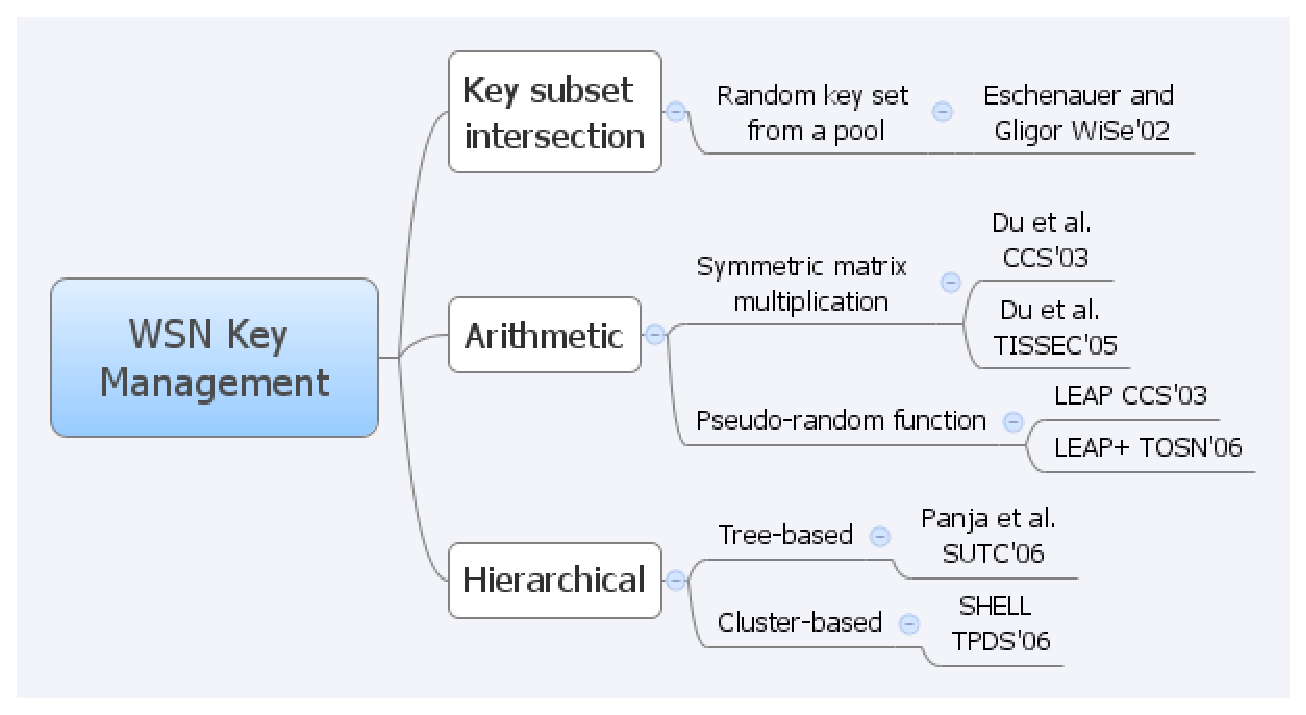
\includegraphics[width=.9\textwidth,keepaspectratio]{wsn_keyman_1}
  \caption{\label{wsn_keyman_1}~WSN~密钥管理协议}
\end{figure}

\begin{enumerate}

\item 密钥子集匹配。为了减少对密钥存储的开销,节点可以仅仅存储部分而不是全网的对密钥信息,当需要通信时,利用子集信息选择或者计算得到通信密钥。密钥子集匹配有两种方案:L. Eschenauer~和~V. Gligor~提出了一个随机密钥子集的方案~\cite{Eschenauer2002}~。首先生成一个密钥池(密钥集),从中随机选择密钥子集存储到每个节点中。当有通信需要时,两个节点查看双方的密钥子集是否有交集,如果有就使用交集中的某密钥通信,否则通过中间节点中转通信;W. Du~等提出一个基于对称矩阵乘法的密钥子集方案~\cite{Du2003}~。

\end{enumerate}


\cite{Perrig2002}

\bibliographystyle{IEEEtran}
\bibliography{IEEEfull,wsn}

\end{document}

